% Created by tikzDevice version 0.10.1 on 2016-08-02 15:20:14
% !TEX encoding = UTF-8 Unicode
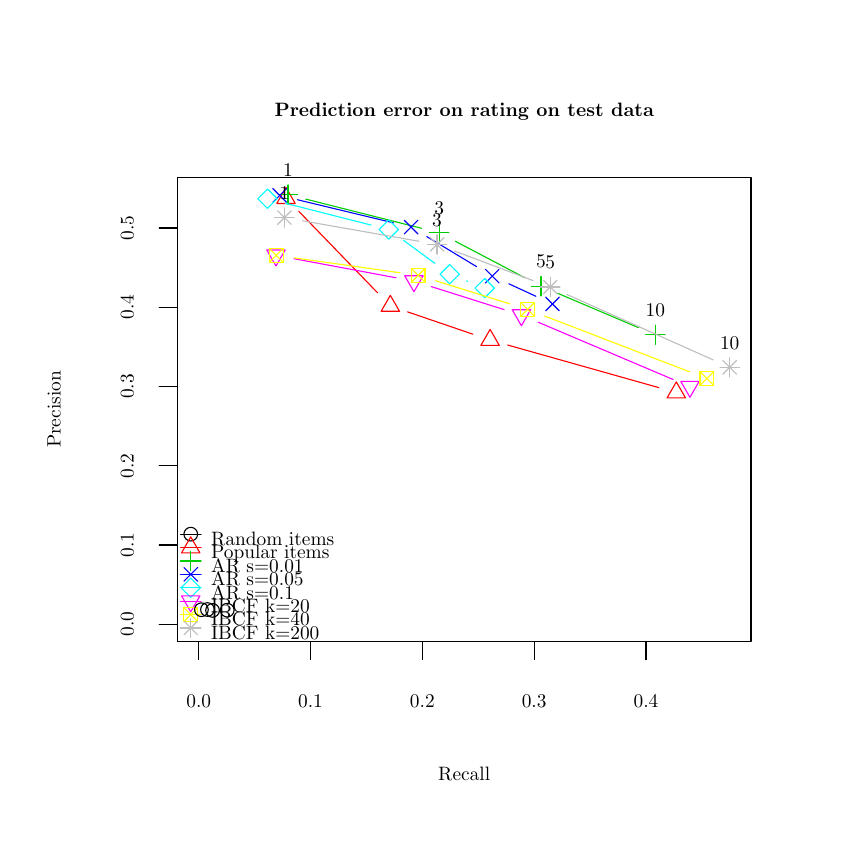
\begin{tikzpicture}[x=1pt,y=1pt]
\definecolor{fillColor}{RGB}{255,255,255}
\path[use as bounding box,fill=fillColor,fill opacity=0.00] (0,0) rectangle (289.08,289.08);
\begin{scope}
\path[clip] (  0.00,  0.00) rectangle (289.08,289.08);
\definecolor{drawColor}{RGB}{0,0,0}

\path[draw=drawColor,line width= 0.4pt,line join=round,line cap=round] ( 61.80, 67.32) -- (223.44, 67.32);

\path[draw=drawColor,line width= 0.4pt,line join=round,line cap=round] ( 61.80, 67.32) -- ( 61.80, 60.72);

\path[draw=drawColor,line width= 0.4pt,line join=round,line cap=round] (102.21, 67.32) -- (102.21, 60.72);

\path[draw=drawColor,line width= 0.4pt,line join=round,line cap=round] (142.62, 67.32) -- (142.62, 60.72);

\path[draw=drawColor,line width= 0.4pt,line join=round,line cap=round] (183.03, 67.32) -- (183.03, 60.72);

\path[draw=drawColor,line width= 0.4pt,line join=round,line cap=round] (223.44, 67.32) -- (223.44, 60.72);

\node[text=drawColor,anchor=base,inner sep=0pt, outer sep=0pt, scale=  0.7] at ( 61.80, 43.56) {0.0};

\node[text=drawColor,anchor=base,inner sep=0pt, outer sep=0pt, scale=  0.7] at (102.21, 43.56) {0.1};

\node[text=drawColor,anchor=base,inner sep=0pt, outer sep=0pt, scale=  0.7] at (142.62, 43.56) {0.2};

\node[text=drawColor,anchor=base,inner sep=0pt, outer sep=0pt, scale=  0.7] at (183.03, 43.56) {0.3};

\node[text=drawColor,anchor=base,inner sep=0pt, outer sep=0pt, scale=  0.7] at (223.44, 43.56) {0.4};

\path[draw=drawColor,line width= 0.4pt,line join=round,line cap=round] ( 54.12, 73.53) -- ( 54.12,216.69);

\path[draw=drawColor,line width= 0.4pt,line join=round,line cap=round] ( 54.12, 73.53) -- ( 47.52, 73.53);

\path[draw=drawColor,line width= 0.4pt,line join=round,line cap=round] ( 54.12,102.16) -- ( 47.52,102.16);

\path[draw=drawColor,line width= 0.4pt,line join=round,line cap=round] ( 54.12,130.79) -- ( 47.52,130.79);

\path[draw=drawColor,line width= 0.4pt,line join=round,line cap=round] ( 54.12,159.42) -- ( 47.52,159.42);

\path[draw=drawColor,line width= 0.4pt,line join=round,line cap=round] ( 54.12,188.06) -- ( 47.52,188.06);

\path[draw=drawColor,line width= 0.4pt,line join=round,line cap=round] ( 54.12,216.69) -- ( 47.52,216.69);

\node[text=drawColor,rotate= 90.00,anchor=base,inner sep=0pt, outer sep=0pt, scale=  0.7] at ( 38.28, 73.53) {0.0};

\node[text=drawColor,rotate= 90.00,anchor=base,inner sep=0pt, outer sep=0pt, scale=  0.7] at ( 38.28,102.16) {0.1};

\node[text=drawColor,rotate= 90.00,anchor=base,inner sep=0pt, outer sep=0pt, scale=  0.7] at ( 38.28,130.79) {0.2};

\node[text=drawColor,rotate= 90.00,anchor=base,inner sep=0pt, outer sep=0pt, scale=  0.7] at ( 38.28,159.42) {0.3};

\node[text=drawColor,rotate= 90.00,anchor=base,inner sep=0pt, outer sep=0pt, scale=  0.7] at ( 38.28,188.06) {0.4};

\node[text=drawColor,rotate= 90.00,anchor=base,inner sep=0pt, outer sep=0pt, scale=  0.7] at ( 38.28,216.69) {0.5};

\path[draw=drawColor,line width= 0.4pt,line join=round,line cap=round] ( 54.12, 67.32) --
	(261.36, 67.32) --
	(261.36,234.96) --
	( 54.12,234.96) --
	( 54.12, 67.32);
\end{scope}
\begin{scope}
\path[clip] (  0.00,  0.00) rectangle (289.08,289.08);
\definecolor{drawColor}{RGB}{0,0,0}

\node[text=drawColor,anchor=base,inner sep=0pt, outer sep=0pt, scale=  0.7] at (157.74, 17.16) {Recall};

\node[text=drawColor,rotate= 90.00,anchor=base,inner sep=0pt, outer sep=0pt, scale=  0.7] at ( 11.88,151.14) {Precision};
\end{scope}
\begin{scope}
\path[clip] ( 54.12, 67.32) rectangle (261.36,234.96);
\definecolor{drawColor}{RGB}{0,0,0}

\path[draw=drawColor,line width= 0.4pt,line join=round,line cap=round] ( 55.23,106.06) -- ( 62.63,106.06);
\definecolor{drawColor}{RGB}{255,0,0}

\path[draw=drawColor,line width= 0.4pt,line join=round,line cap=round] ( 55.23,101.22) -- ( 62.63,101.22);
\definecolor{drawColor}{RGB}{0,205,0}

\path[draw=drawColor,line width= 0.4pt,line join=round,line cap=round] ( 55.23, 96.37) -- ( 62.63, 96.37);
\definecolor{drawColor}{RGB}{0,0,255}

\path[draw=drawColor,line width= 0.4pt,line join=round,line cap=round] ( 55.23, 91.53) -- ( 62.63, 91.53);
\definecolor{drawColor}{RGB}{0,255,255}

\path[draw=drawColor,line width= 0.4pt,line join=round,line cap=round] ( 55.23, 86.69) -- ( 62.63, 86.69);
\definecolor{drawColor}{RGB}{255,0,255}

\path[draw=drawColor,line width= 0.4pt,line join=round,line cap=round] ( 55.23, 81.85) -- ( 62.63, 81.85);
\definecolor{drawColor}{RGB}{255,255,0}

\path[draw=drawColor,line width= 0.4pt,line join=round,line cap=round] ( 55.23, 77.00) -- ( 62.63, 77.00);
\definecolor{drawColor}{RGB}{190,190,190}

\path[draw=drawColor,line width= 0.4pt,line join=round,line cap=round] ( 55.23, 72.16) -- ( 62.63, 72.16);
\definecolor{drawColor}{RGB}{0,0,0}

\path[draw=drawColor,line width= 0.4pt,line join=round,line cap=round] ( 58.93,106.06) circle (  2.47);
\definecolor{drawColor}{RGB}{255,0,0}

\path[draw=drawColor,line width= 0.4pt,line join=round,line cap=round] ( 58.93,105.07) --
	( 62.26, 99.29) --
	( 55.60, 99.29) --
	( 58.93,105.07);
\definecolor{drawColor}{RGB}{0,205,0}

\path[draw=drawColor,line width= 0.4pt,line join=round,line cap=round] ( 55.43, 96.37) -- ( 62.43, 96.37);

\path[draw=drawColor,line width= 0.4pt,line join=round,line cap=round] ( 58.93, 92.87) -- ( 58.93, 99.87);
\definecolor{drawColor}{RGB}{0,0,255}

\path[draw=drawColor,line width= 0.4pt,line join=round,line cap=round] ( 56.46, 89.06) -- ( 61.41, 94.01);

\path[draw=drawColor,line width= 0.4pt,line join=round,line cap=round] ( 56.46, 94.01) -- ( 61.41, 89.06);
\definecolor{drawColor}{RGB}{0,255,255}

\path[draw=drawColor,line width= 0.4pt,line join=round,line cap=round] ( 55.43, 86.69) --
	( 58.93, 90.19) --
	( 62.43, 86.69) --
	( 58.93, 83.19) --
	( 55.43, 86.69);
\definecolor{drawColor}{RGB}{255,0,255}

\path[draw=drawColor,line width= 0.4pt,line join=round,line cap=round] ( 58.93, 78.00) --
	( 62.26, 83.77) --
	( 55.60, 83.77) --
	( 58.93, 78.00);
\definecolor{drawColor}{RGB}{255,255,0}

\path[draw=drawColor,line width= 0.4pt,line join=round,line cap=round] ( 56.46, 74.53) rectangle ( 61.41, 79.48);

\path[draw=drawColor,line width= 0.4pt,line join=round,line cap=round] ( 56.46, 74.53) -- ( 61.41, 79.48);

\path[draw=drawColor,line width= 0.4pt,line join=round,line cap=round] ( 56.46, 79.48) -- ( 61.41, 74.53);
\definecolor{drawColor}{RGB}{190,190,190}

\path[draw=drawColor,line width= 0.4pt,line join=round,line cap=round] ( 56.46, 69.69) -- ( 61.41, 74.64);

\path[draw=drawColor,line width= 0.4pt,line join=round,line cap=round] ( 56.46, 74.64) -- ( 61.41, 69.69);

\path[draw=drawColor,line width= 0.4pt,line join=round,line cap=round] ( 55.43, 72.16) -- ( 62.43, 72.16);

\path[draw=drawColor,line width= 0.4pt,line join=round,line cap=round] ( 58.93, 68.66) -- ( 58.93, 75.66);
\definecolor{drawColor}{RGB}{0,0,0}

\node[text=drawColor,anchor=base west,inner sep=0pt, outer sep=0pt, scale=  0.7] at ( 66.33,101.95) {Random items};

\node[text=drawColor,anchor=base west,inner sep=0pt, outer sep=0pt, scale=  0.7] at ( 66.33, 97.10) {Popular items};

\node[text=drawColor,anchor=base west,inner sep=0pt, outer sep=0pt, scale=  0.7] at ( 66.33, 92.26) {AR s=0.01};

\node[text=drawColor,anchor=base west,inner sep=0pt, outer sep=0pt, scale=  0.7] at ( 66.33, 87.42) {AR s=0.05};

\node[text=drawColor,anchor=base west,inner sep=0pt, outer sep=0pt, scale=  0.7] at ( 66.33, 82.58) {AR s=0.1};

\node[text=drawColor,anchor=base west,inner sep=0pt, outer sep=0pt, scale=  0.7] at ( 66.33, 77.73) {IBCF k=20};

\node[text=drawColor,anchor=base west,inner sep=0pt, outer sep=0pt, scale=  0.7] at ( 66.33, 72.89) {IBCF k=40};

\node[text=drawColor,anchor=base west,inner sep=0pt, outer sep=0pt, scale=  0.7] at ( 66.33, 68.05) {IBCF k=200};

\path[draw=drawColor,line width= 0.4pt,line join=round,line cap=round] ( 62.78, 78.76) circle (  2.47);

\path[draw=drawColor,line width= 0.4pt,line join=round,line cap=round] ( 64.97, 78.82) circle (  2.47);

\path[draw=drawColor,line width= 0.4pt,line join=round,line cap=round] ( 66.80, 78.51) circle (  2.47);

\path[draw=drawColor,line width= 0.4pt,line join=round,line cap=round] ( 72.11, 78.60) circle (  2.47);
\definecolor{drawColor}{RGB}{255,0,0}

\path[draw=drawColor,line width= 0.4pt,line join=round,line cap=round] ( 97.94,222.74) -- (126.45,193.26);

\path[draw=drawColor,line width= 0.4pt,line join=round,line cap=round] (137.29,186.38) -- (160.85,178.33);

\path[draw=drawColor,line width= 0.4pt,line join=round,line cap=round] (173.45,174.40) -- (228.03,159.02);

\path[draw=drawColor,line width= 0.4pt,line join=round,line cap=round] ( 93.35,231.34) --
	( 96.68,225.56) --
	( 90.01,225.56) --
	( 93.35,231.34);

\path[draw=drawColor,line width= 0.4pt,line join=round,line cap=round] (131.04,192.36) --
	(134.37,186.59) --
	(127.71,186.59) --
	(131.04,192.36);

\path[draw=drawColor,line width= 0.4pt,line join=round,line cap=round] (167.10,180.04) --
	(170.43,174.27) --
	(163.76,174.27) --
	(167.10,180.04);

\path[draw=drawColor,line width= 0.4pt,line join=round,line cap=round] (234.38,161.07) --
	(237.71,155.30) --
	(231.04,155.30) --
	(234.38,161.07);
\definecolor{drawColor}{RGB}{0,205,0}

\path[draw=drawColor,line width= 0.4pt,line join=round,line cap=round] (100.45,227.14) -- (142.30,216.58);

\path[draw=drawColor,line width= 0.4pt,line join=round,line cap=round] (154.54,211.90) -- (179.65,198.71);

\path[draw=drawColor,line width= 0.4pt,line join=round,line cap=round] (191.57,193.07) -- (220.72,180.68);

\path[draw=drawColor,line width= 0.4pt,line join=round,line cap=round] ( 90.55,228.75) -- ( 97.55,228.75);

\path[draw=drawColor,line width= 0.4pt,line join=round,line cap=round] ( 94.05,225.25) -- ( 94.05,232.25);

\path[draw=drawColor,line width= 0.4pt,line join=round,line cap=round] (145.20,214.96) -- (152.20,214.96);

\path[draw=drawColor,line width= 0.4pt,line join=round,line cap=round] (148.70,211.46) -- (148.70,218.46);

\path[draw=drawColor,line width= 0.4pt,line join=round,line cap=round] (182.00,195.65) -- (189.00,195.65);

\path[draw=drawColor,line width= 0.4pt,line join=round,line cap=round] (185.50,192.15) -- (185.50,199.15);

\path[draw=drawColor,line width= 0.4pt,line join=round,line cap=round] (223.30,178.10) -- (230.30,178.10);

\path[draw=drawColor,line width= 0.4pt,line join=round,line cap=round] (226.80,174.60) -- (226.80,181.60);
\end{scope}
\begin{scope}
\path[clip] (  0.00,  0.00) rectangle (289.08,289.08);
\definecolor{drawColor}{RGB}{0,0,0}

\node[text=drawColor,anchor=base,inner sep=0pt, outer sep=0pt, scale=  0.7] at ( 94.05,235.35) {1};

\node[text=drawColor,anchor=base,inner sep=0pt, outer sep=0pt, scale=  0.7] at (148.70,221.56) {3};

\node[text=drawColor,anchor=base,inner sep=0pt, outer sep=0pt, scale=  0.7] at (185.50,202.25) {5};

\node[text=drawColor,anchor=base,inner sep=0pt, outer sep=0pt, scale=  0.7] at (226.80,184.70) {10};
\end{scope}
\begin{scope}
\path[clip] ( 54.12, 67.32) rectangle (261.36,234.96);
\definecolor{drawColor}{RGB}{0,0,255}

\path[draw=drawColor,line width= 0.4pt,line join=round,line cap=round] ( 97.49,226.90) -- (132.13,218.56);

\path[draw=drawColor,line width= 0.4pt,line join=round,line cap=round] (144.20,213.60) -- (162.21,202.73);

\path[draw=drawColor,line width= 0.4pt,line join=round,line cap=round] (173.85,196.54) -- (183.65,192.01);

\path[draw=drawColor,line width= 0.4pt,line join=round,line cap=round] ( 88.60,225.97) -- ( 93.55,230.92);

\path[draw=drawColor,line width= 0.4pt,line join=round,line cap=round] ( 88.60,230.92) -- ( 93.55,225.97);

\path[draw=drawColor,line width= 0.4pt,line join=round,line cap=round] (136.07,214.54) -- (141.02,219.49);

\path[draw=drawColor,line width= 0.4pt,line join=round,line cap=round] (136.07,219.49) -- (141.02,214.54);

\path[draw=drawColor,line width= 0.4pt,line join=round,line cap=round] (165.39,196.84) -- (170.34,201.79);

\path[draw=drawColor,line width= 0.4pt,line join=round,line cap=round] (165.39,201.79) -- (170.34,196.84);

\path[draw=drawColor,line width= 0.4pt,line join=round,line cap=round] (187.17,186.76) -- (192.12,191.71);

\path[draw=drawColor,line width= 0.4pt,line join=round,line cap=round] (187.17,191.71) -- (192.12,186.76);
\definecolor{drawColor}{RGB}{0,255,255}

\path[draw=drawColor,line width= 0.4pt,line join=round,line cap=round] ( 93.06,225.64) -- (124.09,217.75);

\path[draw=drawColor,line width= 0.4pt,line join=round,line cap=round] (135.81,212.23) -- (147.17,203.90);

\path[draw=drawColor,line width= 0.4pt,line join=round,line cap=round] (158.63,197.56) -- (159.01,197.41);

\path[draw=drawColor,line width= 0.4pt,line join=round,line cap=round] ( 83.17,227.27) --
	( 86.67,230.77) --
	( 90.17,227.27) --
	( 86.67,223.77) --
	( 83.17,227.27);

\path[draw=drawColor,line width= 0.4pt,line join=round,line cap=round] (126.99,216.13) --
	(130.49,219.63) --
	(133.99,216.13) --
	(130.49,212.63) --
	(126.99,216.13);

\path[draw=drawColor,line width= 0.4pt,line join=round,line cap=round] (149.00,199.99) --
	(152.50,203.49) --
	(156.00,199.99) --
	(152.50,196.49) --
	(149.00,199.99);

\path[draw=drawColor,line width= 0.4pt,line join=round,line cap=round] (161.64,194.97) --
	(165.14,198.47) --
	(168.64,194.97) --
	(165.14,191.47) --
	(161.64,194.97);
\definecolor{drawColor}{RGB}{255,0,255}

\path[draw=drawColor,line width= 0.4pt,line join=round,line cap=round] ( 96.21,205.60) -- (133.08,198.71);

\path[draw=drawColor,line width= 0.4pt,line join=round,line cap=round] (145.87,195.51) -- (172.12,187.21);

\path[draw=drawColor,line width= 0.4pt,line join=round,line cap=round] (184.49,182.64) -- (233.24,161.94);

\path[draw=drawColor,line width= 0.4pt,line join=round,line cap=round] ( 89.73,202.97) --
	( 93.06,208.74) --
	( 86.39,208.74) --
	( 89.73,202.97);

\path[draw=drawColor,line width= 0.4pt,line join=round,line cap=round] (139.57,193.65) --
	(142.91,199.42) --
	(136.24,199.42) --
	(139.57,193.65);

\path[draw=drawColor,line width= 0.4pt,line join=round,line cap=round] (178.41,181.38) --
	(181.74,187.15) --
	(175.08,187.15) --
	(178.41,181.38);

\path[draw=drawColor,line width= 0.4pt,line join=round,line cap=round] (239.31,155.51) --
	(242.65,161.29) --
	(235.98,161.29) --
	(239.31,155.51);
\definecolor{drawColor}{RGB}{255,255,0}

\path[draw=drawColor,line width= 0.4pt,line join=round,line cap=round] ( 96.35,205.89) -- (134.57,200.51);

\path[draw=drawColor,line width= 0.4pt,line join=round,line cap=round] (147.40,197.63) -- (174.34,189.24);

\path[draw=drawColor,line width= 0.4pt,line join=round,line cap=round] (186.80,184.90) -- (239.26,164.69);

\path[draw=drawColor,line width= 0.4pt,line join=round,line cap=round] ( 87.34,204.34) rectangle ( 92.29,209.29);

\path[draw=drawColor,line width= 0.4pt,line join=round,line cap=round] ( 87.34,204.34) -- ( 92.29,209.29);

\path[draw=drawColor,line width= 0.4pt,line join=round,line cap=round] ( 87.34,209.29) -- ( 92.29,204.34);

\path[draw=drawColor,line width= 0.4pt,line join=round,line cap=round] (138.63,197.11) rectangle (143.58,202.06);

\path[draw=drawColor,line width= 0.4pt,line join=round,line cap=round] (138.63,197.11) -- (143.58,202.06);

\path[draw=drawColor,line width= 0.4pt,line join=round,line cap=round] (138.63,202.06) -- (143.58,197.11);

\path[draw=drawColor,line width= 0.4pt,line join=round,line cap=round] (178.16,184.80) rectangle (183.11,189.75);

\path[draw=drawColor,line width= 0.4pt,line join=round,line cap=round] (178.16,184.80) -- (183.11,189.75);

\path[draw=drawColor,line width= 0.4pt,line join=round,line cap=round] (178.16,189.75) -- (183.11,184.80);

\path[draw=drawColor,line width= 0.4pt,line join=round,line cap=round] (242.94,159.84) rectangle (247.89,164.79);

\path[draw=drawColor,line width= 0.4pt,line join=round,line cap=round] (242.94,159.84) -- (247.89,164.79);

\path[draw=drawColor,line width= 0.4pt,line join=round,line cap=round] (242.94,164.79) -- (247.89,159.84);
\definecolor{drawColor}{RGB}{190,190,190}

\path[draw=drawColor,line width= 0.4pt,line join=round,line cap=round] ( 99.28,219.30) -- (141.42,211.89);

\path[draw=drawColor,line width= 0.4pt,line join=round,line cap=round] (154.09,208.42) -- (182.65,197.69);

\path[draw=drawColor,line width= 0.4pt,line join=round,line cap=round] (194.85,192.67) -- (247.66,169.05);

\path[draw=drawColor,line width= 0.4pt,line join=round,line cap=round] ( 90.30,217.97) -- ( 95.25,222.92);

\path[draw=drawColor,line width= 0.4pt,line join=round,line cap=round] ( 90.30,222.92) -- ( 95.25,217.97);

\path[draw=drawColor,line width= 0.4pt,line join=round,line cap=round] ( 89.28,220.45) -- ( 96.28,220.45);

\path[draw=drawColor,line width= 0.4pt,line join=round,line cap=round] ( 92.78,216.95) -- ( 92.78,223.95);

\path[draw=drawColor,line width= 0.4pt,line join=round,line cap=round] (145.44,208.27) -- (150.39,213.22);

\path[draw=drawColor,line width= 0.4pt,line join=round,line cap=round] (145.44,213.22) -- (150.39,208.27);

\path[draw=drawColor,line width= 0.4pt,line join=round,line cap=round] (144.42,210.74) -- (151.42,210.74);

\path[draw=drawColor,line width= 0.4pt,line join=round,line cap=round] (147.92,207.24) -- (147.92,214.24);

\path[draw=drawColor,line width= 0.4pt,line join=round,line cap=round] (186.35,192.89) -- (191.30,197.84);

\path[draw=drawColor,line width= 0.4pt,line join=round,line cap=round] (186.35,197.84) -- (191.30,192.89);

\path[draw=drawColor,line width= 0.4pt,line join=round,line cap=round] (185.33,195.37) -- (192.33,195.37);

\path[draw=drawColor,line width= 0.4pt,line join=round,line cap=round] (188.83,191.87) -- (188.83,198.87);

\path[draw=drawColor,line width= 0.4pt,line join=round,line cap=round] (251.21,163.88) -- (256.16,168.83);

\path[draw=drawColor,line width= 0.4pt,line join=round,line cap=round] (251.21,168.83) -- (256.16,163.88);

\path[draw=drawColor,line width= 0.4pt,line join=round,line cap=round] (250.18,166.36) -- (257.18,166.36);

\path[draw=drawColor,line width= 0.4pt,line join=round,line cap=round] (253.68,162.86) -- (253.68,169.86);
\end{scope}
\begin{scope}
\path[clip] (  0.00,  0.00) rectangle (289.08,289.08);
\definecolor{drawColor}{RGB}{0,0,0}

\node[text=drawColor,anchor=base,inner sep=0pt, outer sep=0pt, scale=  0.7] at ( 92.78,227.05) {1};

\node[text=drawColor,anchor=base,inner sep=0pt, outer sep=0pt, scale=  0.7] at (147.92,217.34) {3};

\node[text=drawColor,anchor=base,inner sep=0pt, outer sep=0pt, scale=  0.7] at (188.83,201.97) {5};

\node[text=drawColor,anchor=base,inner sep=0pt, outer sep=0pt, scale=  0.7] at (253.68,172.96) {10};

\node[text=drawColor,anchor=base,inner sep=0pt, outer sep=0pt, scale=  0.7] at (157.74,257.07) {\bfseries Prediction error on rating on test data};
\end{scope}
\end{tikzpicture}
